\documentclass{article} 
\usepackage{graphicx}
\usepackage[francais]{babel} 
\usepackage[utf8]{inputenc}
\usepackage[T1]{fontenc} 
\usepackage{amsmath} 
\usepackage{amsfonts}
\usepackage{verbatim} 
\usepackage{float} 
\usepackage{hyperref}
\usepackage{scrtime}
\usepackage[scale=2]{ccicons}
\usepackage{tabularx}
\usepackage{Sweave}
\begin{document}
\Sconcordance{concordance:serie1-solutions.tex:/home/francois/ACT-2010-Exercices/serie1-solutions.Rnw:%
1 13 1 1 0 8 1 1 2 1 0 3 1 3 0 1 2 1 1 1 2 20 0 1 8 7 1 1 2 19 0 1 2 1 %
7 7 1 1 2 19 0 1 2 1 7 9 1 1 2 19 0 1 2 1 1 1 2 19 0 1 2 1 1 1 2 19 0 1 %
2 1 1 1 2 1 0 1 1 10 0 1 1 3 0 1 3 19 0 1 2 1 10 7 1 1 2 1 0 2 1 7 0 1 %
2 2 1 1 2 1 0 1 1 3 0 1 2 37 1}


\section{Méthodes de lissage et saisonnalité}
\label{sec:serie-dexercices-1}

\subsection{Noël s'en vient !}
\label{sec:exercice-1-1}

\begin{Schunk}
\begin{Sinput}
> library(xtable) # Librairie contenant la fonction xtable permettant de 
>                                         #générer des tables an LaTeX
> library(TTR) ## Librairie contenant les outils de lissage de données
> Yt <- read.csv("inflation.csv",header=TRUE,sep="\t")[,2] ## Importer les données
> Yt.ts <-ts(Yt,start=c(2008,7),deltat=1/12) ## Définir la série chronologique
\end{Sinput}
\end{Schunk}

\textbf{Tableau des données} 
\begin{Schunk}
\begin{Sinput}
> xtable(Yt.ts,digits=1) ## Générer une table LaTeX
\end{Sinput}
% latex table generated in R 2.15.2 by xtable 1.7-1 package
% Mon Oct  7 22:26:51 2013
\begin{table}[ht]
\centering
\begin{tabular}{rrrrrrrrrrrrr}
  \hline
 & Jan & Feb & Mar & Apr & May & Jun & Jul & Aug & Sep & Oct & Nov & Dec \\ 
  \hline
2008 &  &  &  &  &  &  & -0.1 & 0.5 & 0.7 & 0.9 & 1.4 & 2.3 \\ 
  2009 & 1.5 & 0.9 & 2.2 & 0.8 & 0.2 & 0.3 & 1.0 & 0.3 & 0.8 & 0.4 & 1.6 & 2.0 \\ 
  2010 & 3.2 & 2.3 & 1.4 & 0.6 & 0.7 & 1.1 & -0.2 & 1.4 & 0.9 & 1.4 & 1.4 & 1.9 \\ 
  2011 & 3.1 & 2.1 & 2.7 & 1.7 & 1.7 & 0.1 & 0.9 & 1.6 & 1.6 & 2.5 & 2.4 & 2.6 \\ 
  2012 & 2.0 & 3.2 & 2.9 & 1.4 & 1.1 & 1.3 & 1.4 & 1.4 & 1.5 & 1.7 & 2.3 & 2.4 \\ 
  2013 & 3.0 & 2.3 & 2.3 & 1.9 & 1.7 & 0.5 & 0.9 &  &  &  &  &  \\ 
   \hline
\end{tabular}
\end{table}\end{Schunk}
\begin{figure}[p]
  \centering
  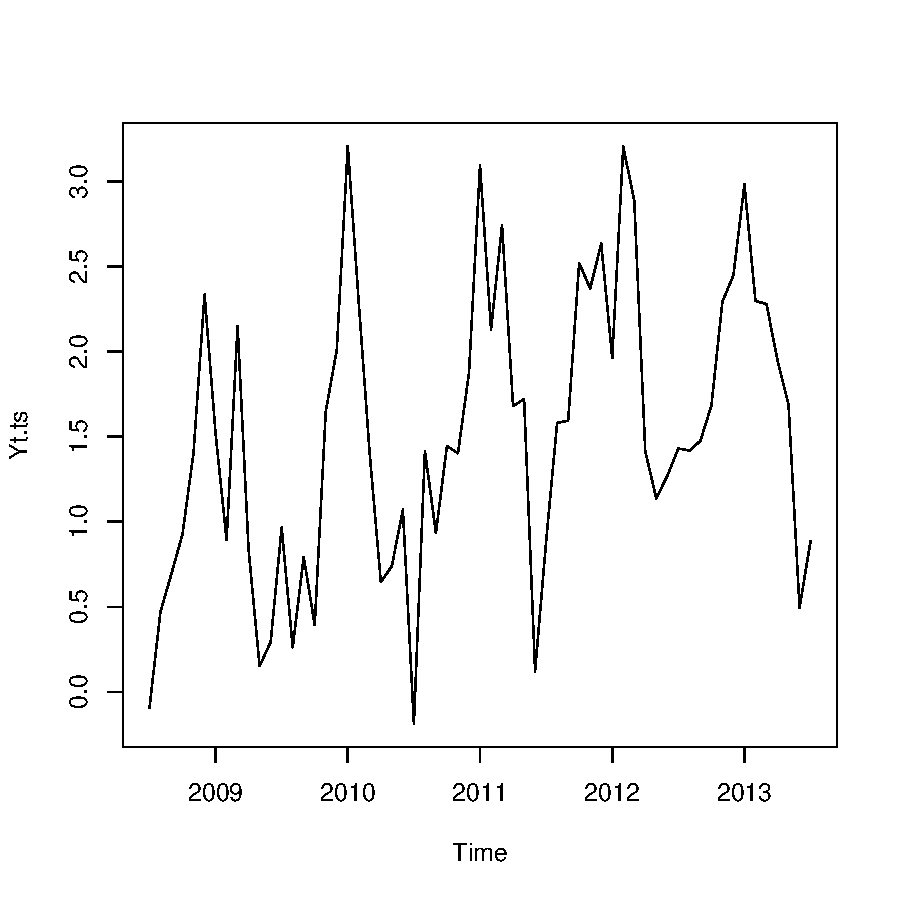
\includegraphics[height=4in, width=4in]{exercice1-graph1.pdf}
  \caption{Graphique de la série $Y_t$}
  \label{fig:exercice1-graph1}
\end{figure}

\textbf{Élimination de la saisonnalité}
\begin{Schunk}
\begin{Sinput}
> xtable(Zt.ts <- diff(Yt.ts,12),digits=1)
\end{Sinput}
% latex table generated in R 2.15.2 by xtable 1.7-1 package
% Mon Oct  7 22:26:51 2013
\begin{table}[ht]
\centering
\begin{tabular}{rrrrrrrrrrrrr}
  \hline
 & Jan & Feb & Mar & Apr & May & Jun & Jul & Aug & Sep & Oct & Nov & Dec \\ 
  \hline
2009 &  &  &  &  &  &  & 1.1 & -0.2 & 0.1 & -0.5 & 0.2 & -0.3 \\ 
  2010 & 1.7 & 1.4 & -0.8 & -0.2 & 0.6 & 0.8 & -1.2 & 1.2 & 0.1 & 1.1 & -0.2 & -0.1 \\ 
  2011 & -0.1 & -0.2 & 1.4 & 1.0 & 1.0 & -0.9 & 1.1 & 0.2 & 0.7 & 1.1 & 1.0 & 0.8 \\ 
  2012 & -1.1 & 1.1 & 0.1 & -0.3 & -0.6 & 1.1 & 0.5 & -0.2 & -0.1 & -0.8 & -0.1 & -0.2 \\ 
  2013 & 1.0 & -0.9 & -0.6 & 0.5 & 0.5 & -0.8 & -0.5 &  &  &  &  &  \\ 
   \hline
\end{tabular}
\end{table}\end{Schunk}

\begin{figure}[p]
  \centering
  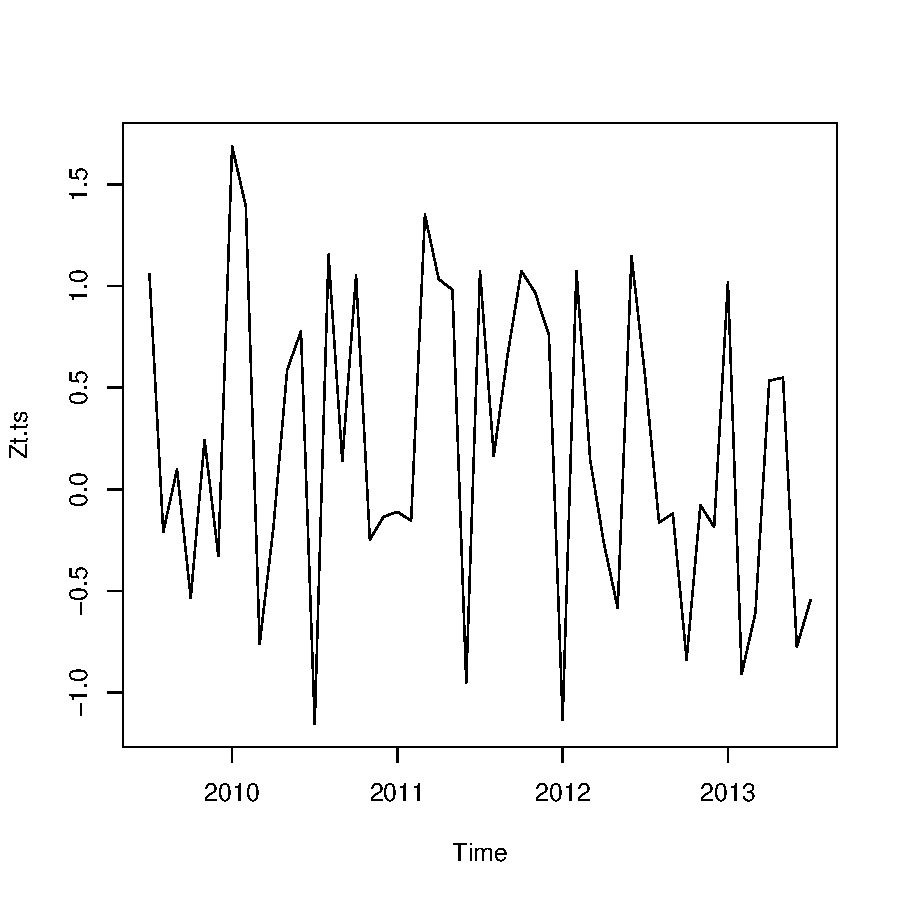
\includegraphics[height=4in, width=4in]{exercice1-graph2.pdf}
  \caption{Graphique de la série désaisonnalisée $Z_t$}
  \label{fig:exercice1-graph2}
\end{figure}

\textbf{Composante de saisonnalité}
\begin{Schunk}
\begin{Sinput}
> xtable(Yt.ts-Zt.ts,digits=1)
\end{Sinput}
% latex table generated in R 2.15.2 by xtable 1.7-1 package
% Mon Oct  7 22:26:51 2013
\begin{table}[ht]
\centering
\begin{tabular}{rrrrrrrrrrrrr}
  \hline
 & Jan & Feb & Mar & Apr & May & Jun & Jul & Aug & Sep & Oct & Nov & Dec \\ 
  \hline
2009 &  &  &  &  &  &  & -0.1 & 0.5 & 0.7 & 0.9 & 1.4 & 2.3 \\ 
  2010 & 1.5 & 0.9 & 2.2 & 0.8 & 0.2 & 0.3 & 1.0 & 0.3 & 0.8 & 0.4 & 1.6 & 2.0 \\ 
  2011 & 3.2 & 2.3 & 1.4 & 0.6 & 0.7 & 1.1 & -0.2 & 1.4 & 0.9 & 1.4 & 1.4 & 1.9 \\ 
  2012 & 3.1 & 2.1 & 2.7 & 1.7 & 1.7 & 0.1 & 0.9 & 1.6 & 1.6 & 2.5 & 2.4 & 2.6 \\ 
  2013 & 2.0 & 3.2 & 2.9 & 1.4 & 1.1 & 1.3 & 1.4 &  &  &  &  &  \\ 
   \hline
\end{tabular}
\end{table}\end{Schunk}

\begin{figure}[p]
  \centering
  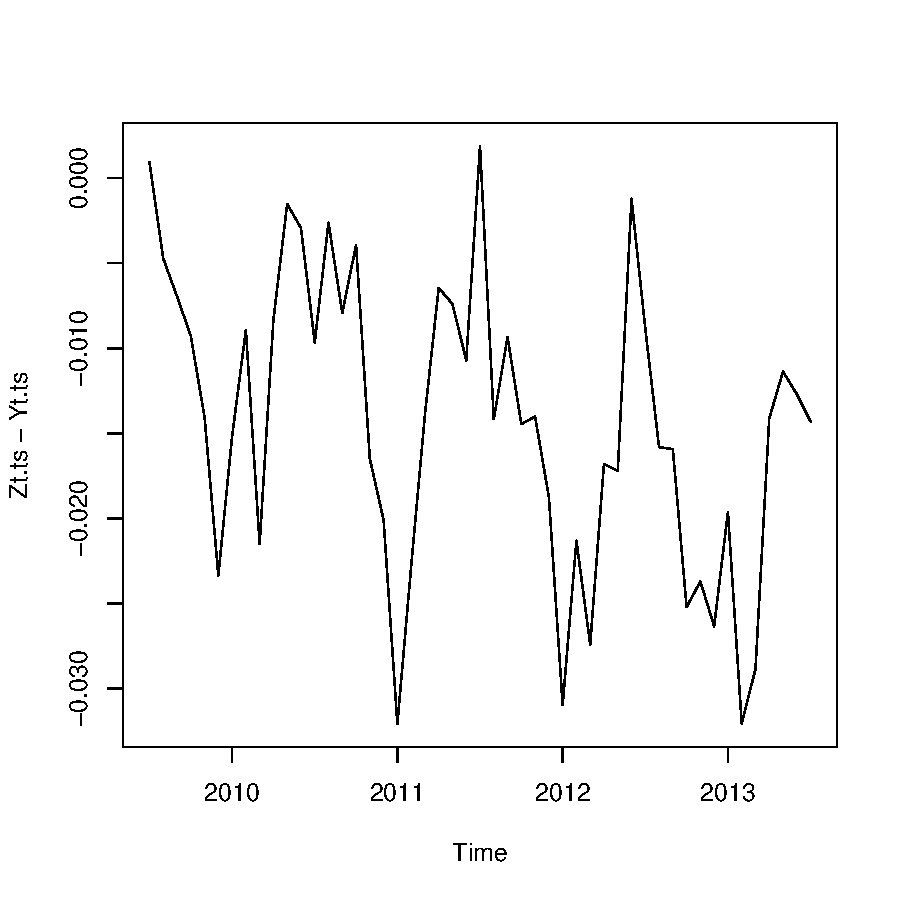
\includegraphics[height=4in, width=4in]{exercice1-graph3.pdf}
  \caption{Graphique de la composante de saisonnalité $Y_t-Z_t$}
  \label{fig:exercice1-graph3}
\end{figure}
\clearpage
\textbf{Élimination de la tendance}

Moyenne mobile avec $q=1$. Comme la fonction \emph{SMA()} utilise les $2q+1$ 
données précédentes et que nous voulons une moyenne mobile centrée, nous devons utiliser l'opérateur de rétrodécalage $B()$ pour décaler la série.

\begin{Schunk}
\begin{Sinput}
> xtable(mt1 <- lag(SMA(Zt.ts,n=3),1),digits=2) ## Simple Moving Average(q=1)
\end{Sinput}
% latex table generated in R 2.15.2 by xtable 1.7-1 package
% Mon Oct  7 22:26:51 2013
\begin{table}[ht]
\centering
\begin{tabular}{rrrrrrrrrrrrr}
  \hline
 & Jan & Feb & Mar & Apr & May & Jun & Jul & Aug & Sep & Oct & Nov & Dec \\ 
  \hline
2009 &  &  &  &  &  &  &  & 0.32 & -0.22 & -0.06 & -0.21 & 0.54 \\ 
  2010 & 0.92 & 0.77 & 0.15 & -0.12 & 0.39 & 0.07 & 0.26 & 0.05 & 0.78 & 0.32 & 0.22 & -0.16 \\ 
  2011 & -0.13 & 0.36 & 0.74 & 1.12 & 0.36 & 0.37 & 0.10 & 0.63 & 0.63 & 0.90 & 0.93 & 0.20 \\ 
  2012 & 0.23 & 0.03 & 0.32 & -0.24 & 0.10 & 0.37 & 0.51 & 0.09 & -0.37 & -0.34 & -0.37 & 0.25 \\ 
  2013 & -0.02 & -0.16 & -0.33 & 0.16 & 0.10 & -0.26 &  &  &  &  &  &  \\ 
   \hline
\end{tabular}
\end{table}\end{Schunk}
\clearpage 
Moyenne mobile avec $q=5$
\begin{Schunk}
\begin{Sinput}
> xtable(mt2 <- lag(SMA(Zt.ts,n=11),5),digits=2) ## Simple Moving Average(q=5)
\end{Sinput}
% latex table generated in R 2.15.2 by xtable 1.7-1 package
% Mon Oct  7 22:26:51 2013
\begin{table}[ht]
\centering
\begin{tabular}{rrrrrrrrrrrrr}
  \hline
 & Jan & Feb & Mar & Apr & May & Jun & Jul & Aug & Sep & Oct & Nov & Dec \\ 
  \hline
2009 &  &  &  &  &  &  &  &  &  &  &  & 0.28 \\ 
  2010 & 0.25 & 0.17 & 0.26 & 0.32 & 0.40 & 0.40 & 0.24 & 0.10 & 0.16 & 0.30 & 0.34 & 0.36 \\ 
  2011 & 0.37 & 0.37 & 0.37 & 0.33 & 0.45 & 0.55 & 0.63 & 0.54 & 0.52 & 0.44 & 0.32 & 0.36 \\ 
  2012 & 0.36 & 0.40 & 0.32 & 0.22 & 0.05 & -0.02 & 0.06 & 0.06 & -0.04 & -0.07 & 0.03 & -0.02 \\ 
  2013 & -0.14 & -0.18 &  &  &  &  &  &  &  &  &  &  \\ 
   \hline
\end{tabular}
\end{table}\end{Schunk}
\clearpage 
Lissage exponentiel double avec $\alpha=0.75$
\begin{Schunk}
\begin{Sinput}
> xtable(mt3 <- DEMA(Zt.ts,n=1,ratio=.05),digits=2) ## Double Exponential 
\end{Sinput}
% latex table generated in R 2.15.2 by xtable 1.7-1 package
% Mon Oct  7 22:26:51 2013
\begin{table}[ht]
\centering
\begin{tabular}{rrrrrrrrrrrrr}
  \hline
 & Jan & Feb & Mar & Apr & May & Jun & Jul & Aug & Sep & Oct & Nov & Dec \\ 
  \hline
2009 &  &  &  &  &  &  & 1.06 & 0.94 & 0.85 & 0.71 & 0.66 & 0.55 \\ 
  2010 & 0.65 & 0.72 & 0.57 & 0.48 & 0.48 & 0.50 & 0.33 & 0.39 & 0.36 & 0.41 & 0.33 & 0.28 \\ 
  2011 & 0.22 & 0.17 & 0.27 & 0.33 & 0.38 & 0.24 & 0.31 & 0.29 & 0.31 & 0.38 & 0.43 & 0.45 \\ 
  2012 & 0.29 & 0.36 & 0.33 & 0.26 & 0.17 & 0.25 & 0.27 & 0.22 & 0.18 & 0.07 & 0.04 & 0.01 \\ 
  2013 & 0.09 & -0.02 & -0.09 & -0.04 & 0.00 & -0.09 & -0.14 &  &  &  &  &  \\ 
   \hline
\end{tabular}
\end{table}\begin{Sinput}
>                                                   ## Moving Average
\end{Sinput}
\end{Schunk}
\clearpage 
Régression linéaire
\begin{Schunk}
\begin{Sinput}
> t <- 0:48
> (lm1 <- lm(Zt.ts~t)) ## Modèle de régression sur une variable
\end{Sinput}
\begin{Soutput}
Call:
lm(formula = Zt.ts ~ t)

Coefficients:
(Intercept)            t  
   0.446924    -0.009856  
\end{Soutput}
\begin{Sinput}
> coeff1 <- coefficients(lm1)
\end{Sinput}
\end{Schunk}
\begin{Schunk}
\begin{Sinput}
> xtable(mt4 <- ts(coeff1[1]+t*coeff1[2],start=c(2009,7),deltat=1/12),digits=2)
\end{Sinput}
% latex table generated in R 2.15.2 by xtable 1.7-1 package
% Mon Oct  7 22:26:51 2013
\begin{table}[ht]
\centering
\begin{tabular}{rrrrrrrrrrrrr}
  \hline
 & Jan & Feb & Mar & Apr & May & Jun & Jul & Aug & Sep & Oct & Nov & Dec \\ 
  \hline
2009 &  &  &  &  &  &  & 0.45 & 0.44 & 0.43 & 0.42 & 0.41 & 0.40 \\ 
  2010 & 0.39 & 0.38 & 0.37 & 0.36 & 0.35 & 0.34 & 0.33 & 0.32 & 0.31 & 0.30 & 0.29 & 0.28 \\ 
  2011 & 0.27 & 0.26 & 0.25 & 0.24 & 0.23 & 0.22 & 0.21 & 0.20 & 0.19 & 0.18 & 0.17 & 0.16 \\ 
  2012 & 0.15 & 0.14 & 0.13 & 0.12 & 0.11 & 0.10 & 0.09 & 0.08 & 0.07 & 0.06 & 0.05 & 0.04 \\ 
  2013 & 0.03 & 0.02 & 0.01 & 0.00 & -0.01 & -0.02 & -0.03 &  &  &  &  &  \\ 
   \hline
\end{tabular}
\end{table}\end{Schunk}
\clearpage 
\begin{figure}[p]
  \centering
  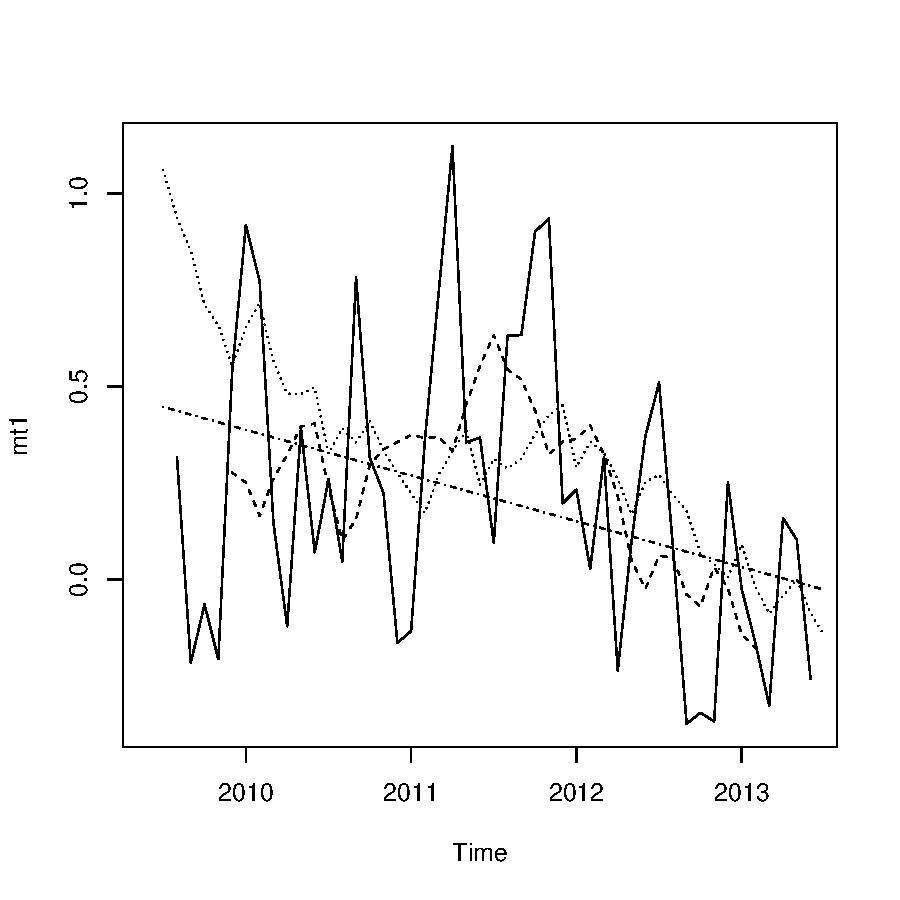
\includegraphics[height=4in, width=4in]{exercice1-graph4.pdf}
  \caption{Graphique de la tendance $m_t$}
  \label{fig:exercice1-graph4}
\end{figure}
\clearpage 
\textbf{Projection du taux d'inflation}
\begin{Schunk}
\begin{Sinput}
> projection <- coeff1[1]+53*coeff1[2]
> saisonnalite <- mean((Yt.ts-Zt.ts)[6+12*0:3])
> (taux.inf.dec.2013 <- (projection+saisonnalite))
\end{Sinput}
\begin{Soutput}
(Intercept) 
   2.137743 
\end{Soutput}
\end{Schunk}
Le taux d'inflation prejeté en décembre 2013 est 2.14\%\\

\textbf{Solution du problème}
\begin{Schunk}
\begin{Sinput}
> depense.dec.2008 <- 674
> depense.dec.2013 <- 674*(1+taux.inf.dec.2013/100)
\end{Sinput}
\end{Schunk}
Le montant projeté des achats de cadeaux en décembre 2013 est 688.41 \$

\clearpage 
\subsection{Incendies}

On remarque d'abord que $q=2$.

On peut ensuite poser les équations suivantes:
\begin{align}
  \label{eq:1}
  4+3+a+b+2 &= 24\\
  b+2+4+6+c &= 26\\
  c+0+2+8+3 &= 19
\end{align}

En résolvant, on obtient la solution.\\

\textbf{Solution:}\\

\begin{tabular}{|l|l|l|}
\hline
\multicolumn{1}{|l|}{Mois} & \multicolumn{1}{l|}{Incendies} & \multicolumn{1}{l|}{Moyenne Mobile} \\ \hline
1 & 4 & \multicolumn{1}{l|}{-} \\ \hline
2 & 3 & \multicolumn{1}{l|}{-} \\ \hline
3 & \textbf{7} & 4,8 \\ \hline
4 & \textbf{8} & 4,8 \\ \hline
5 & 2 & 5,4 \\ \hline
6 & 4 & 5,2 \\ \hline
7 & 6 & 3,6 \\ \hline
8 & \textbf{6} & 3,6 \\ \hline
9 & 0  & 4,4 \\ \hline
10 & 2 & 3,8 \\ \hline
11 & 8 & \multicolumn{1}{l|}{-} \\ \hline
12 & 3 & \multicolumn{1}{l|}{-} \\ \hline
\end{tabular}

\clearpage

\subsection{Option de vente}

\begin{Schunk}
\begin{Sinput}
> rf <- 0.0175
> rB <- rf+0.02
> S0 <- 10.46
> ST <- 8.73
> K <- S0*exp(rf*84/365)
> bbry <- read.csv("blackberry.csv",header=TRUE,sep=";")
> bbry.sel <- bbry[as.POSIXlt(bbry$Date)$wday==5,][1+3:12*4,]$Close 
>                                         #Extraire le prix un vendredi sur 4
> l.bbry.sel <- log(bbry.sel)
> (diff.l.bbry.sel <- diff(l.bbry.sel)) 
\end{Sinput}
\begin{Soutput}
[1]  0.288637639  0.112996047 -0.061344651 -0.103095509 -0.017497594
[6] -0.086523113  0.005008358 -0.340978628 -0.090637274
\end{Soutput}
\begin{Sinput}
>                                         #On obtient la série des rendements
>                                         #mensuels
> (mu.diff.l.bbry.sel <- mean(diff.l.bbry.sel))
\end{Sinput}
\begin{Soutput}
[1] -0.03260386
\end{Soutput}
\begin{Sinput}
> (sigma.diff.l.bbry.sel <- sd(diff.l.bbry.sel))
\end{Sinput}
\begin{Soutput}
[1] 0.170735
\end{Soutput}
\begin{Sinput}
>                                         #Moyenne et écart-type des rendements 
>                                         #mensuels
> (prix.arbre <- S0*(ud <- exp(3*(mu.diff.l.bbry.sel+c(1,-1)*
+                                 sigma.diff.l.bbry.sel/(2*sqrt(3))))))
\end{Sinput}
\begin{Soutput}
[1] 10.996838  8.181586
\end{Soutput}
\begin{Sinput}
>                                         #Prix de l'arbre binomial
> (p.rn <- (exp(rf*84/365)-ud[2])/(ud[1]-ud[2]))
\end{Sinput}
\begin{Soutput}
[1] 0.8243048
\end{Soutput}
\begin{Sinput}
>                                         #Probabilité neutre au risque
> q.rn <- 1-p.rn
> (P0 <- sum(exp(-rf*84/365)*(c(p.rn,q.rn)*pmax(K-prix.arbre,0))))
\end{Sinput}
\begin{Soutput}
[1] 0.406084
\end{Soutput}
\begin{Sinput}
>                                         #Prix de l'option de vente
> (BT <- P0*exp(rB*84/365)) #Montant emprunté avec intérêts
\end{Sinput}
\begin{Soutput}
[1] 0.4096037
\end{Soutput}
\begin{Sinput}
> (K-ST)-BT  #Profit
\end{Sinput}
\begin{Soutput}
[1] 1.362608
\end{Soutput}
\end{Schunk}

La valeur du paramètre $\mu$ de rendement moyen est -0.0326.
La valeur du paramètre $\sigma$ de volatilité est 0.1707.
La valeur des prix de l'arbre binomial sont 10.9968 et 8.1816.
La valeur de la probabilité neutre au risque d'une hausse est 0.8243.
La valeur de l'option est 0.4061.
Le profit, qui correspont à la différence entre la réclamation contingente de l'option et le coût d'acquisition, est de 1.3626.

\clearpage

\subsection{Lissage exponentiel I}

On calcule d'abord les deux séries lissées \\

\begin{tabular}{|l|r|r|}
\hline
\multicolumn{1}{|c|}{$\mathcal{A}$} & $\alpha=0,4$ & $\alpha=0,7$ \\ \hline
1,2 & 1,2000 & 1,2000 \\ \hline
1,5 & 1,3200 & 1,4100 \\ \hline
1,4 & 1,3520 & 1,4030 \\ \hline
2,1 & 1,6512 & 1,8909 \\ \hline
1,8 & 1,7107 & 1,8273 \\ \hline
1,9 & 1,7864 & 1,8782 \\ \hline
2,2 & 1,9519 & 2,1035 \\ \hline
2,4 & 2,1311 & 2,3110 \\ \hline
2,0 & 2,0787 & 2,0933 \\ \hline
1,9 & 2,0072 & 1,9580 \\ \hline
\end{tabular} \\

On évalue ensuite l'erreur quadratique pour chaque terme \\

\begin{tabular}{|l|r|r|}
\hline
\multicolumn{1}{|c|}{$\mathcal{A}$} & \multicolumn{1}{l|}{$SE(\alpha=0,4)$} & \multicolumn{1}{l|}{$SE(\alpha=0,7)$} \\ \hline
1,2 & \multicolumn{1}{l|}{} & \multicolumn{1}{l|}{} \\ \hline
1,5 & 0,0324 & 0,0081 \\ \hline
1,4 & 0,0023 & 0,0000 \\ \hline
2,1 & 0,2014 & 0,0437 \\ \hline
1,8 & 0,0080 & 0,0007 \\ \hline
1,9 & 0,0129 & 0,0005 \\ \hline
2,2 & 0,0616 & 0,0093 \\ \hline
2,4 & 0,0723 & 0,0079 \\ \hline
2,0 & 0,0062 & 0,0087 \\ \hline
1,9 & 0,0115 & 0,0034 \\ \hline
\end{tabular} \\

On obtient enfin l'erreur quadratique moyenne\\

\begin{tabular}{|l|l|l|}
\hline
 & $\alpha=0,4$ & $\alpha=0,7$ \\ \hline
MSE & \multicolumn{1}{r|}{0,0454} & \multicolumn{1}{r|}{0,0092} \\ \hline
\end{tabular} \\

Les calculs effectués se trouvent dans le fichier \url{Lissage.Exponentiel.I.ods} \footnote{Ce fichier est au format OpenDocument et s'ouvre avec la plupart des suites bureautiques}.

Avec R, on obtient les résultats suivants en utilisant la fonction de lissage exponentiel \emph{EMA()}.

\begin{Schunk}
\begin{Sinput}
> A <- c(1.2, 1.5, 1.4, 2.1, 1.8, 1.9, 2.2, 2.4, 2.0, 1.9)
> n.A <- length(A)
> A.EMA.4 <- EMA(A,n=1,ratio=0.4)
> A.EMA.7 <- EMA(A,n=1,ratio=0.7)
> A.SE <- (A-cbind(A.EMA.4,A.EMA.7))^2
> cbind(A,A.EMA.4,A.EMA.7,A.SE)
\end{Sinput}
\begin{Soutput}
        A  A.EMA.4  A.EMA.7     A.EMA.4      A.EMA.7
 [1,] 1.2 1.200000 1.200000 0.000000000 0.0000000000
 [2,] 1.5 1.320000 1.410000 0.032400000 0.0081000000
 [3,] 1.4 1.352000 1.403000 0.002304000 0.0000090000
 [4,] 2.1 1.651200 1.890900 0.201421440 0.0437228100
 [5,] 1.8 1.710720 1.827270 0.007970918 0.0007436529
 [6,] 1.9 1.786432 1.878181 0.012897691 0.0004760688
 [7,] 2.2 1.951859 2.103454 0.061573857 0.0093210722
 [8,] 2.4 2.131116 2.311036 0.072298864 0.0079145417
 [9,] 2.0 2.078669 2.093311 0.006188861 0.0087069216
[10,] 1.9 2.007202 1.957993 0.011492180 0.0033632189
\end{Soutput}
\begin{Sinput}
> (A.MSE <- colMeans(A.SE)*(n.A/(n.A-1)))
\end{Sinput}
\begin{Soutput}
   A.EMA.4    A.EMA.7 
0.04539420 0.00915081 
\end{Soutput}
\end{Schunk}

La valeur $\alpha=0.7$ produit une erreur quadratique moyenne inférieure.

\subsection{Lissage exponentiel II}

Une solution assez simple est d'utiliser le solveur intégré au logiciel tableau que vous utilisez et d'optimiser la valeur de la cellule contenant $\alpha$ avec comme critère de minimisation la cellule contenant l'erreur quadratique moyenne (MSE).

On peut aussi construire une fonction d'optimisation dans R qui réplique le comportement du chiffrier que nous avons construit dans le logiciel tableur.

\begin{Schunk}
\begin{Sinput}
> funOptAlphaDEMA <- function(alpha,data)
+   {
+     data.n <- length(data)
+     data.DEMA <- DEMA(A,n=1,ratio=alpha)
+     data.SE <- (data-data.DEMA)^2
+     data.MSE <- mean(data.SE)*data.n/(data.n-1)
+     print(c(data.MSE,alpha))
+     data.MSE
+   }
> optimize(funOptAlphaDEMA,c(0.4,0.7),A)
\end{Sinput}
\begin{Soutput}
[1] 0.006416607 0.514589803
[1] 0.003674206 0.585410197
[1] 0.002489337 0.629179607
[1] 0.001912478 0.656230590
[1] 0.001607733 0.672949017
[1] 0.001437559 0.683281573
[1] 0.001338969 0.689667444
[1] 0.00128047 0.69361413
[1] 0.001245226 0.696053315
[1] 0.001223788 0.697560814
[1] 0.001210668 0.698492500
[1] 0.001202609 0.699068314
[1] 0.001197648 0.699424186
[1] 0.001194588 0.699644128
[1] 0.0011927 0.6997801
[1] 0.001191534 0.699864069
[1] 0.001190814 0.699915990
[1] 0.00119025 0.69995669
[1] 0.00119025 0.69995669
$minimum
[1] 0.6999567

$objective
[1] 0.00119025
\end{Soutput}
\end{Schunk}

Tout comme pour le lissage exponentiel effectué à la question précédente, la valeur $\alpha=0.7$ produit une erreur quadratique moyenne inférieure.

\subsection{Bank of America (calculatrice et informatique)}

On importe d'abord l'ensemble de données
\begin{Schunk}
\begin{Sinput}
> BoA <- ts(read.csv("BoA.csv",header=TRUE,sep="\t"))
\end{Sinput}
\end{Schunk}

\begin{enumerate}
\item 
  On trace ensuite le corrélogramme (figure \ref{fig:exercice1.6-graph1})
  La fonction \emph{acf} nous permet d'afficher un corrélogramme
\begin{figure}[p]
  \centering
  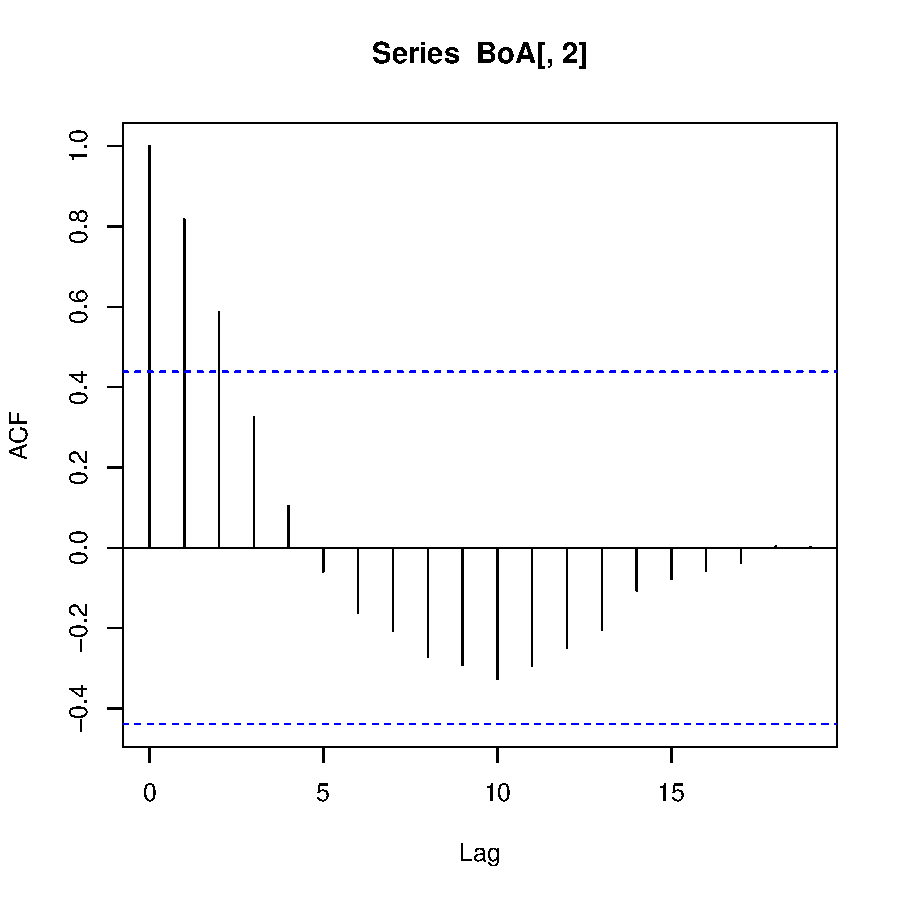
\includegraphics[height=4in, width=4in]{exercice1-6-graph1}
  \caption{Corrélogramme de la série BoA}
  \label{fig:exercice1.6-graph1}
\end{figure}

La fonction d'autocorrélation empirique $\hat{\rho}$ prend les valeurs suivantes
\begin{Schunk}
\begin{Sinput}
> (BoA.acf <- acf(BoA[,2],lag.max=19))
\end{Sinput}
\begin{Soutput}
Autocorrelations of series ‘BoA[, 2]’, by lag

     0      1      2      3      4      5      6      7      8      9     10 
 1.000  0.817  0.587  0.325  0.105 -0.059 -0.161 -0.207 -0.272 -0.291 -0.325 
    11     12     13     14     15     16     17     18     19 
-0.293 -0.249 -0.203 -0.106 -0.078 -0.057 -0.038  0.003  0.002 
\end{Soutput}
\begin{Sinput}
> dummy <- dev.off()
\end{Sinput}
\end{Schunk}

En utilisant la méthode vue dans le cours, on construit un intervalle de confiance au niveau $1-\alpha=0.9$ à partir de la distribution normale. La valeur de $n$ est 20.

\begin{Schunk}
\begin{Sinput}
> (BoA.acf.IC <- round(c(1/sqrt(20)*qnorm(0.05),-1/sqrt(20)*qnorm(0.05)),4))
\end{Sinput}
\begin{Soutput}
[1] -0.3678  0.3678
\end{Soutput}
\end{Schunk}

\begin{align*}
  IC &= \frac{1}{\sqrt{n}}\left[-z_{\alpha / 2},z_{\alpha / 2} \right] \\
  &= \frac{1}{\sqrt{20}}\left[-z_{0.05},z_{0.05} \right] \\
  &= \left[ -0.3678,0.3678 \right]
\end{align*}

\begin{Schunk}
\begin{Sinput}
> sum(BoA.acf$acf<BoA.acf.IC[1]) + sum(BoA.acf$acf>BoA.acf.IC[2])
\end{Sinput}
\begin{Soutput}
[1] 3
\end{Soutput}
\end{Schunk}
Comme 3 valeurs sur 20, soit 15\% de celles-ci, sont à l'extérieur de l'intervalle de confiance, alors on doit rejeter l'hypothèse selon laquelle la série est stationnaire lorsqu'on se base sur le test du corrélogramme.
\item
  Ici, on n'a qu'à tracer la série et compter les changements de direction (figure \ref{fig:exercice1.6-graph2})
\begin{figure}[p]
  \centering
  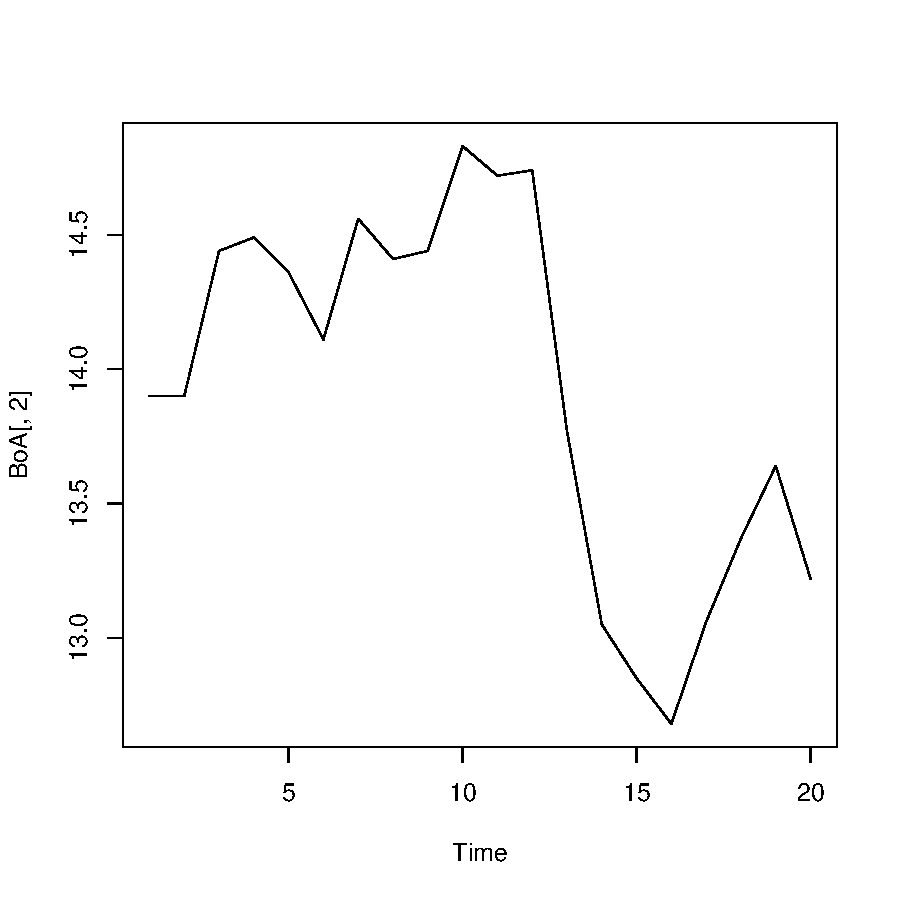
\includegraphics[height=4in, width=4in]{exercice1-6-graph2}
  \caption{Corrélogramme de la série BoA}
  \label{fig:exercice1.6-graph2}
\end{figure}

On en dénombre 9.

\begin{Schunk}
\begin{Sinput}
> BoA.chdir <- abs((9-(2/3)*18)/sqrt((16*20-29)/90))
> BoA.chdir > qnorm(0.95)
\end{Sinput}
\begin{Soutput}
[1] TRUE
\end{Soutput}
\end{Schunk}
On évalue la statistique de test, qui prend la valeur 1.6684. Comme cette valeur est supérieure au seuil de 1.6449, on rejette l'hypothèse de stationnarité avec le test du changement de direction.
\item
\begin{Schunk}
\begin{Sinput}
> Box.test(BoA[,2],lag=19,type="Ljung-Box")
\end{Sinput}
\begin{Soutput}
	Box-Ljung test

data:  BoA[, 2] 
X-squared = 52.1457, df = 19, p-value = 6.292e-05
\end{Soutput}
\begin{Sinput}
> qchisq(0.9,19)
\end{Sinput}
\begin{Soutput}
[1] 27.20357
\end{Soutput}
\end{Schunk}

On rejette l'hypothèse de stationnarité car la valeur de $Q^{*}=52.1457$ est supérieure au quantile $\chi^2_{0.1}(19) = 27.20357$
  
\item
  Les tests sont indépendants, différents entre eux et ne sont pas équivalents car leurs statistiques ne suivent pas la même distribution asymptotique.
  
\item
\begin{Schunk}
\begin{Sinput}
> round(diff(log(BoA[,2])),4)
\end{Sinput}
\begin{Soutput}
Time Series:
Start = 2 
End = 20 
Frequency = 1 
 [1]  0.0000  0.0381  0.0035 -0.0090 -0.0176  0.0314 -0.0104  0.0021  0.0267
[10] -0.0074  0.0014 -0.0681 -0.0537 -0.0154 -0.0133  0.0295  0.0235  0.0200
[19] -0.0313
\end{Soutput}
\end{Schunk}

\item
\begin{Schunk}
\begin{Sinput}
> (BoA.hist.var <- na.trim(apply(cbind(BoA[,2],lag(BoA[,2],1),lag(BoA[,2],2),lag(BoA[,2],3),lag(BoA[,2],4)),
+       1,
+       var)))
\end{Sinput}
\begin{Soutput}
 [1] 0.08642 0.06185 0.03017 0.02963 0.02753 0.06795 0.03257 0.03617 0.18785
[10] 0.61597 0.79813 0.71857 0.17257 0.06697 0.15075 0.12818
\end{Soutput}
\begin{Sinput}
> Box.test(BoA.hist.var,lag=15,type="Ljung-Box")
\end{Sinput}
\begin{Soutput}
	Box-Ljung test

data:  BoA.hist.var 
X-squared = 19.9483, df = 15, p-value = 0.1739
\end{Soutput}
\begin{Sinput}
> qchisq(0.9,15)
\end{Sinput}
\begin{Soutput}
[1] 22.30713
\end{Soutput}
\end{Schunk}

On remarque que la série des volatilités historiques avec $q=2$ est stationnaire bien que la volatilité ne soit pas constante.
  
\end{enumerate}

\clearpage
\subsection{Variance d'une série non-stationnaire}

La variance du $t^e$ terme est équivalente à la somme de la variance des $t$ premiers termes d'erreurs. La différence entre les variances des $5^e$ terme et du $7^e$ terme est donc égale à la somme:
\begin{align*}
  \label{eq:2}
  V\left[\epsilon_6\right]+V\left[\epsilon_7\right] &= 0.1(6^2+7^2) \\
  & = 8.5
\end{align*}


\clearpage


\includegraphics[height=7mm,keepaspectratio=true]{by-sa}\\
Cette création est mise à disposition selon le contrat
\href{http://creativecommons.org/licenses/by-sa/2.5/ca/deed.fr}{%
  Paternité-Partage à l'identique 2.5 Canada} de Creative Commons
disponible à l'adresse \\
http://creativecommons.org/licenses/by-sa/2.5/ca/deed.fr \\

En vertu de ce contrat, vous êtes libre de:

\begin{itemize}
\item \textbf{partager} --- reproduire, distribuer et communiquer
  l'{\oe}uvre;
\item \textbf{remixer} --- adapter l'{\oe}uvre;
\item utiliser cette {\oe}uvre à des fins commerciales.
\end{itemize}

Selon les conditions suivantes:\\

  \begin{tabularx}{\linewidth}{@{}lX@{}}
    \raisebox{-9mm}[0mm][13mm]{%
      
\includegraphics[height=11mm,keepaspectratio=true]{by}} &
    \textbf{Attribution} --- Vous devez attribuer l'{\oe}uvre de la
    manière indiquée par l'auteur de l'{\oe}uvre ou le titulaire des
    droits (mais pas d'une manière qui suggérerait qu'ils vous
    soutiennent ou
    approuvent votre utilisation de l'{\oe}uvre). \\
    \raisebox{-9mm}{
\includegraphics[height=11mm,keepaspectratio=true]{sa}}
    & \textbf{Partage à l'identique} --- Si vous modifiez, transformez
    ou adaptez cette {\oe}uvre, vous n'avez le droit de distribuer
    votre création que sous une licence identique ou similaire à
    celle-ci.
  \end{tabularx}
\clearpage
Document généré le \today \ à \ \thistime 
\end{document}
